\chapter{Methods and Results}

TODO:\begin{enumerate}
    \item Check for consistent notation
\end{enumerate}

\section{Description}

\subsection*{Model and Synthetic Data Simulations}

\begin{figure}[htbp]
    \centering
    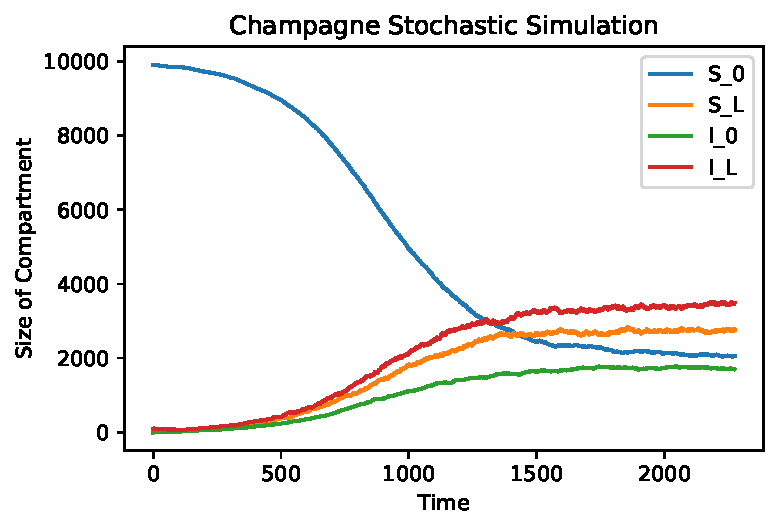
\includegraphics{../champagne_GP_images/champagne_simulation.pdf}
    \caption{A Doob-Gillespie Simulation of the model described by \cite{champagne_using_2022}.}\label{fig:champ_doob}
\end{figure}

In order to trial this method we used the model described in
\cite{champagne_using_2022}, and graphically depicted in Figure
\ref{fig:champ_diag}. Exact model simulations such as in Figure
\ref{fig:champ_doob} were computed using the
Doob-Gillespie algorithm (Algorithm \ref{alg:doob}).

Synthetic data was generated from a single run of the model, using a population
size of 1,000, an initial infected population of 10 (with both liver and blood
stage infection). The parameters used closely followed those reported in
\cite{champagne_using_2022}: \begin{itemize}
    \item effective blood stage treatment proportion $\alpha = 0.4,$
    \item effective liver stage treatment proportion $\beta = 0.4,$
    \item rate of liver stage disease clearance $\gamma_L = 1 / 223 \text{ days}^{-1},$
    \item importation rate $\delta = 0$ (assumed to be known),
    \item rate of infection $\lambda = 0.04 \text{ days}^{-1},$
    \item rate of relapse $f = 1 / 72 \text{ days}^{-1},$
    \item rate of blood stage disease clearance $r = 1 / 60 \text{ days}^{-1}.$
\end{itemize}
To generate the synthetic data, the model was run for 30 days and at least 15,000 events
(infections, recoveries etc.), after which time, it was assumed to have reached
equilibrium.

\subsection*{Summary Statistics and Discrepancy Function}

The synthetic data (as summary statistics) we measured were:
\begin{enumerate}
    \item prevalence at the end of the model run - $p_\text{obs},$
    \item number of cases in the first week of the epidemic
          (first month incidence) - $m_\text{obs},$
    \item a single observation of the number of weekly cases at equilibrium
          (weekly incidence) - $w_\text{obs}.$
\end{enumerate} Similarly we extracted $p, m,$ and $w$ from each new model run.

Our discrepency function we used was the $L_2$ norm of the relative differences
$$
    \mathcal{D}(\alpha, \beta, \gamma_L, \lambda, f, r) = \sqrt{
        \left(\frac{p - p_\text{obs}}{p_\text{obs}}\right)^2
        + \left(\frac{m - m_\text{obs}}{m_\text{obs}}\right)^2
        + \left(\frac{w - w_\text{obs}}{w_\text{obs}}\right)^2
    }.
$$
Relative differences were chosen to limit the impact between the scale
differences of the summary statistics. No systematic comparison of norms was done.

\begin{table}[htbp]
    \centering
    \begin{tabular}{c |c |c}
        Parameter                                                     & Bound & Unit   \\
        \hline
        Proportion of treatment clearing blood stage disease $\alpha$ & 1     &        \\
        Proportion of treatment clearing liver stage disease $\beta$  & 1     &        \\
        Rate of liver stage disease clearance $\gamma_L$              & 1/30  & 1/days \\
        Rate of infection $\lambda$                                   & 1/10  & 1/days \\
        Rate of relapse $f$                                           & 1/14  & 1/days \\
        Rate of blood stage disease clearance $r$                     & 1/14  & 1/days
    \end{tabular}
    \caption{Target parameters to be estimated and their upper bounds, derived from \cite{champagne_using_2022, white_variation_2016}.}
    \label{table:param_bounds}
\end{table}

All parameters were given conservative upper bounds after considering
values reported in the literature.

\subsection*{Gaussian Process Setup}

To approximate the true discrepancy function, a Gaussian process with constant
mean $\mu_{\mathcal{GP}}$, and 5/2 Mat\'ern kernel was used with automatic
relevance determination - i.e.\ each parameter $\theta\in\bm{\theta}$ was
scaled by $\ell_\theta,$ such
that the kernel is
$$
    k(\bm{\theta}_i, \bm{\theta}_i^\prime)
    = \sigma_a^2 (1 + z_i + \frac{z_i^2}{3})\exp(-z_i)
$$
where
$$
    z_i = \sqrt{
        5 \sum_{\theta\in \bm{\theta}}\left(
        \frac{\theta_i - \theta_i^\prime}{\ell_\theta}
        \right)^2
    }.
$$ and $\sigma_O^2$ is the observation variance.

\subsection*{Initialisation}

50 Latin hypercube samples that were scaled to the upper bounds described in
Table \ref{table:param_bounds} were taken, and for each set of parameters, two
model run discrepencies were taken. The hyper\-parameters
$\sigma_O^2, \sigma_a^2, \ell_\alpha, \ell_\beta, \ell_{\gamma_L}, \ell_\lambda, \ell_f,$
and $\ell_r$ were chosen by maximising the leave one out predictive
log-probability as described in \cite[116]{rasmussen_gaussian_2008}.

The acquisition function used was
$$\mu(\bm\theta) - \eta_t\sqrt{\mathrm{v}(\bm\theta)}$$
with $\eta_t:= \sqrt{2\ln(\frac{t^{2d + 2}\pi^2}{3\varepsilon})},$ and
$\varepsilon \in (0, 1)$ that can be chosen
(with a lower epsilon resulting in more exploration), $\mu(\bm\theta)$ and
$\mathrm{v}(\bm\theta)$ are the posterior mean and variance.
$\varepsilon = 0.1$ was used.
$$(\mu_\text{min} - \mu(\bm\theta))
    \varPhi\left(
    \frac{\mu_\text{min} - \mu(\bm\theta)}{\sqrt{\mathrm{v}(\bm\theta)}}
    \right) + \sqrt{\mathrm{v}(\bm\theta)}
    \phi\left(
    \frac{\mu_\text{min} - \mu(\bm\theta)}{\sqrt{\mathrm{v}(\bm\theta)}}
    \right)$$
$\mu_\text{min} := \min_{\bm{\theta}} \mu(\bm\theta)$
$\varPhi, \phi$

\subsection*{Justification}

Using relative differences limits the impact between the scale differences of
the summary statistics.

\section{Running the Model and Our Choices}

Although most of the procedure we used closely follows the paper by
\cite{gutmann_bayesian_2016}, there are a few key ways in which we modified the
manuscript's method. In particular, we felt the choice of squared exponential
kernel was not a good assumption, since it implicitly assumes a high degree of
smoothness in the target discrepency function. This is unlikely to be met if
the model has any bifurcation points. To compensate for any non-smoothness in
the function, the length scale is forced to be set very small. Therefore,
although the squared exponential is the most commonly chosen kernel,
we used a Mat\'ern kernel with $\nu = 5/2$. This is not as constrained as a
squared exponential kernel, but realisations are twice mean square
differentiable.

A constant mean was used, rather than the quadratic mean, because the
parameters are well bounded, and we don't need to worry about what happens when
they go to infinity. Post-hoc mean fitting could be done on the discrepencies
sampled space in order to extend the likelihood into regions that haven't been
tested without reverting to the mean function.

There seems to be a mistake in \cite{gutmann_bayesian_2016}, where the
exploration parameters is written as
$\eta_t:= \sqrt{2\ln(\frac{t^{2d + 2}\pi^2}{3\varepsilon})}.$ This seems to be
inherited from \cite{brochu_tutorial_2010}. We use Brochu's original citation
\cite{srinivas_gaussian_2010} to revise this to
$\eta_t:= \sqrt{2\ln(\frac{t^{2d + 2}\pi^2}{3\varepsilon})}.$
\footnote{One Python package that implements BOLFI notes this error, see:
    \url{https://github.com/elfi-dev/elfi/blob/dev/elfi/methods/bo/acquisition.py}}

The Gaussian process and Gaussian process regression was implemented using
TensorFlow in Python \cite{abadi_tensorflow_2015}.

\section{Results}

